\textbf{Problem 22.} \\
\hrule 

Refer to exercise 13, and calculate and graph the cdf. Then use it to calculate the probabilities of the events given in parts (a)-(d) of that problem. 

\begin{table}[h]
\begin{tabular}{lll}
\hline
x & $P[X = x]$ & $P[X \leq x]$ \\ \hline
0 & .1 & .1 \\
1 & .15 & .25 \\
2 & .2 & .45 \\
3 & .25 & .7 \\
4 & .2 & .9 \\
5 & .06 & .96 \\
6 & .04 & 1 \\
\multicolumn{1}{}{} & 
\end{tabular}
\end{table}

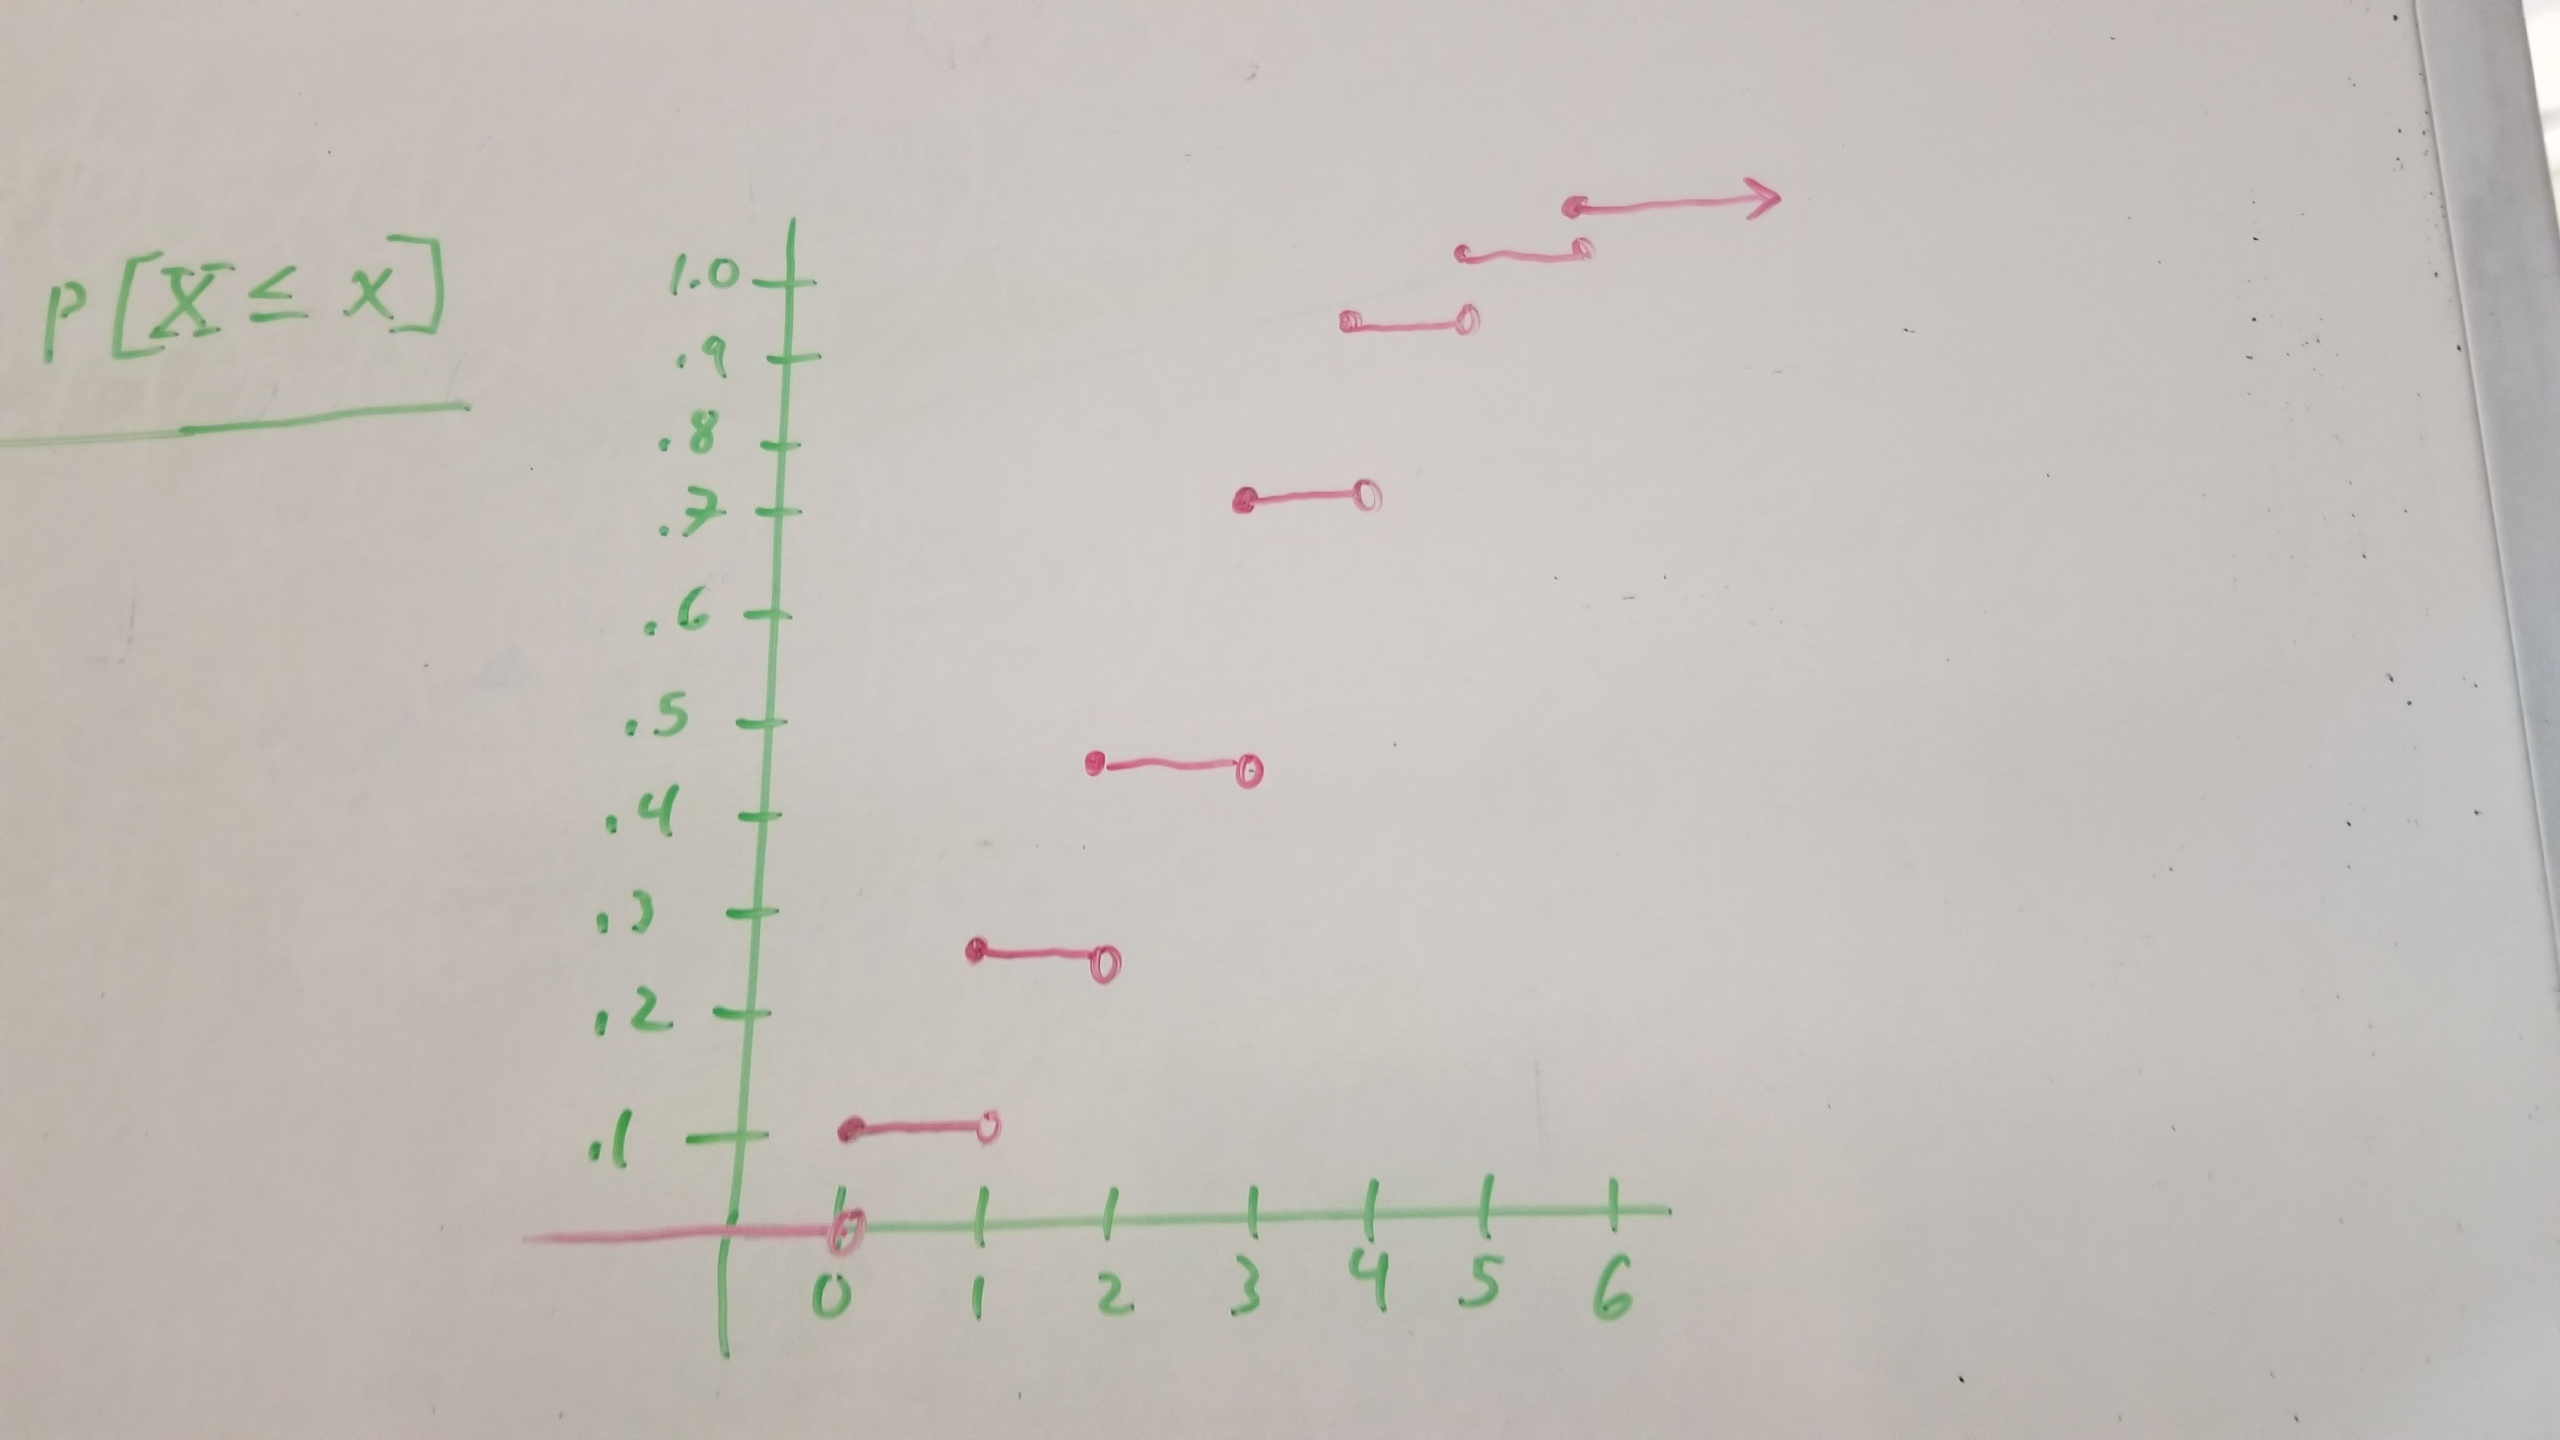
\includegraphics[scale=0.125]{images/whw4/3.2.22.jpg}

\textbf{a.} $P[X \leq 3] = \boxed{.7}$

\textbf{b.} $P[X < 3] = P[X \leq 2] = \boxed{.45}$

\textbf{c.} $P[X \geq 3] = 1 - P[X \leq 3] = \boxed{.55}$

\textbf{d.} $P[2 \leq X \leq 5] = P[X \leq 5] - P[X \leq 1] = \boxed{.71}$